\documentclass[12pt, letterpaper]{report}
\usepackage[utf8]{inputenc}
\usepackage[margin=1in]{geometry}
\usepackage[spanish]{babel}
\usepackage{graphicx}
\graphicspath{ {Images/} }
\title{Proyecto 1: Colecciones en Java}
\author{Zarate García Zuriel, Rosales López Luis André, Núñez Quintana Luis Axel}
\date{15 de noviembre, 2020}

\begin{document}
\title{Proyecto 1: Ordenamiento Externo}
	\begin{titlepage}
		\begin{center}
			\textsc{\Large Universidad Nacional Autónoma de México}\\
			\textsc{\large Facultad de Ingeniería}\\[2em]
			\begin{figure}[h]
				\begin{center}
					
\includegraphics[scale=0.50]{unamLogo.jpg}
				\end{center}
			\end{figure}
			\vspace{1em}
			\textsc{\huge \textbf{Proyecto 1: Ordenamiento Externo}}\\[2em]
			\textsc{\Large Estructura de Datos y Algoritmos II}\\[1em]
			\textsc{\large Grupo 09}\\[1em]
			\textsc{\Large Equipo 3}\\[1em]
			\textsc{Núñez Quintana Luis Axel}\\[1em]
			\textsc{Rosales López Luis André}\\[1em]
			\textsc{Zarate García Zuriel}
		\end{center}
		\vspace*{\fill}
		\textsc{Ciudad de México \hspace*{\fill}15 de noviembre, 2020}
	\end{titlepage}
    
    \section*{Objetivos}
    Que el alumno implemente los algoritmos de ordenamiento externo, que conozca elementos para el manejo de archivos, aplique los conceptos generales de programación y desarrolle sus habilidades de trabajo en equipo.
    
    \section*{Introducción}
    El ser humano ha descubierto la necesidad de ordenar las cosas para distintos propósitos: buscar con mayor facilidad un objeto, comprender mejor el funcionamiento de un sistema o por simple estética. \\
    
    Un ejemplo del uso del ordenamiento para facilitar la búsqueda: Encontrar un número $x$ entre 100 números distintos. Si están ordenados, será fácil encontrarlo, si no, se requiere una "vista de águila" para lograrlo.\\
    
    Un ejemplo del uso del ordenamiento en la comprensión del funcionamiento de un sistema: El estudio de la biología requiere clasificar y ordenar todas las formas de vida existentes en nuestro planeta. Para poder comprender el comportamiento de una especie específica respecto a su reproducción, respiración, genética, anatomía, fisiología, etc., requiere de un ordenamiento. \\
    
    Un ejemplo de el uso del ordenamiento con fines estéticos: En la arquitectura, música, poesía, literatura y en el cine se utiliza el ordenamiento constantemente. También la presentación de nuestro hogar se ve influenciada por esta operación tan necesaria, ya que "se ve feo" si tenemos desorden en las diferentes habitaciones.\\
    
    El ordenamiento se ha vuelto extremadamente necesario en la era de la computación, ya que requerimos manejar cantidades enormes de información de distinto tipo y de distintas personas al rededor de todo el mundo. Sin ese orden tan necesario, encontrar cualquier información que nos interese en internet nos llevaría muchísimo tiempo, gestionar un sistema de inscripciones escolares sería una labor titánica y encontrar nuestra información más importante en nuestros ordenadores (valga la redundancia) no sería tan fácil. Es por ello que los algorítmos de ordenamiento nos han facilitado mucho las cosas hasta el día de hoy.\\
    
    Hay dos tipos de algorítmos de ordenamiento: Interno y externo. Los algorítmos de ordenamiento interno se llevan a cabo en memoria principal (RAM). Por otro lado, los algorítmos de ordenamiento externo se llevan a cabo en memoria secundaria (Hard Disk O SSD). En el presente reporte, analizamos y codificamos tres algorítmos de ordenamiento externo en el lenguaje de programación orientado a objetos Java: Radix externo, Polifase y Mezcla Equilibrada. Llevamos a cabo cada uno de estos con archivos que contienen la información de alumnos de la UNAM  estructurada de la siguiente manera: \\
    
        \begin{center}
            \textit{Nombre(s), Apellidos, Número de cuenta}
        \end{center}
    \section*{Algoritmos de ordenamiento externo: análisis}
    
    \subsection*{Mezcla equilibrada}
    En esta implementación se hace una simulación de Mezcla Equilibrada, ya que no utiliza los archivos auxiliares para volverlos a leer y sobreescribir el archivo original con las claves ordenadas. Sin embargo, es útil para fines didácticos, ya que podemos ver un archivo con las iteraciones realizadas, los archivos auxiliares y el archivo final, donde se encuentran las claves ya ordenadas.\\
    
    A grandes rasgos, el algorítmo se lleva a cabo en los siguientes pasos: 
    
        \begin{enumerate}
        
            \item Se lee el archivo ``original.txt''. 
            \item La información de cada elemento se introduce en una lista ligada.
            \item Se realiza la primer fase con dicha lista, la cual consiste en separar toda la información en sublistas (bloques) que se colocan en dos archivos auxiliares $Archivo A$ y $Archivo B$ de manera alternada. Estos bloques se ``leen'' de los archivos auxiliares y se mezclan (de manera ordenada), formando bloques más grandes. En realidad, estos archivos auxiliares se mantienen como listas ligadas de las listas ligadas (para simular los bloques) durante la ejecución.
            \item Se realiza la segunda fase, en la cual se vuelven a separar los bloques más grandes y se vuelven a mezclar de manera iterativa hasta que se tenga una lista de tamaño 1 (es decir, hasta que todos los bloques han sido mezclados y ordenados). Al final, se devuelve la lista ordenada.
            \item Finalmente, se escribe en el archivo final las claves ordenadas y se retorna la ruta del archivo para indicarle su localización al usuario.
            
        \end{enumerate}
    
    Ahora, veamos en qué consisten cada uno de estos pasos. \\
    
     \textbf{Paso 0.}\\
    De una clase llamada ``Utilidades'' tomamos un método para crear directorios llamado ``inicializarDir()''. Con este método, creamos la carpeta ``Mezcla Equilibrada'' dentro de la carpeta ``Archivos Ordenamientos''. Dentro de esta nueva carpeta, se crea otra carpeta que toma el nombre de la forma de ordenamiento que ha elegido el usuario (por nombre, apellido o número de cuenta). Si esta carpeta ya existe (de una ejecución anterior), se vacía su contenido, si no existe, se crea. Dentro de ``Ordenamiento por...'', se crean los archivos ``iteraciones.txt'' y ``Mezcla Equilibrada terminada'', así como otra carpeta donde están los archivos auxiliares $ArchivoA$ y $ArchivoB$.\\
    
    \begin{figure}[h!]
		\begin{center}
			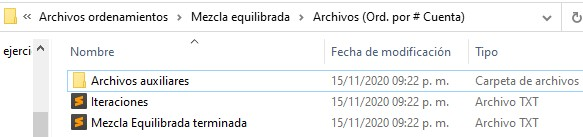
\includegraphics[scale=1]{D1.jpg}
			\caption{Creación de carpetas en Mezcla Equilibrada.}
		\end{center}
	\end{figure}
    
    \newpage
    
    \textbf{Paso 1.}\\
    Primero, se obtiene el path complto (absoluto) del archivo ``original.txt'' y se lee con el método ``readFile()'', que pertenece a la clase auxiliar ``Archivos''. Esta información se guarda en un arreglo de Strings, donde cada elemento del arreglo tiene la forma \textit{Nombre(s), Apellidos, Número de cuenta}.\\
    
    \textbf{Paso 2.}\\
    Después, con ayuda de un ciclo, se introduce cada elemento en una lista ligada de Strings y se pasa su referencia a los métodos pertinentes.\\
    
    \textbf{Paso 3.}\\
    Para separar los bloques, utilizamos un método llamado ``bloque()'', que toma la lista original e introduce en una lista auxiliar los elementos de dicha lista hasta que deje de estar ordenada. Al final de este método, se agrega el índice en el que se quedó el recorrido como un String y se devuelve la lista auxiliar. Este método es llamado en el método ``primeraFase()´´ constantemente hasta que se termina de recorrer la lista original, donde, en cada llamada del método ``bloque()'' se introduce el valor de retorno de forma alterna en dos listas de listas: $ListaA$ y $ListaB$ (que simula a los archivos $ArchivoA$ y $ArchivoB$). Al final de esta primera fase, los métodos se mezclan y ordenan con un breve \textit{Merge Sort.}, que es implementado en el método ``mezcla()''. El resultado de esta mezcla es introducido en una lista de listas $listaC$.\\
    
    \textbf{Paso 4.}\\
    La segunda fase toma como valor de entrada la lista que retorna la primera fase y separan los bloques mezclados en nuevas listas de listas $ListaA$ y $listaB$ (que simulan la sobreescritura de los archivos $ArchivoA$ y $ArchivoB$). Para esto, se realiza un ciclo que separa los bloques impares en la lista superior y los pares en los bloques inferiores. Una vez separados, se invoca al método ``mezcla()'' para mezclar los bloques de la lista superior con los de la lista inferior. Esta mezcla vuelve a introducirse en la lista recibida originalmente: $listaC$. Una vez terminada la iteración, se borran todos los elementos de las listas auxiliares $listaA$ y $ListaB$ y se repite la iteración con la misma $listaC$. Esto es, hasta que la $listaC$ es de tamaño 1, es decir, hasta que se tiene un solo bloque dentro de la lista.\\
    
    \newpage
    
    \textbf{Paso 5.}\\
    Este último paso está ligado a todos los pasos anteriores (incluyendo el 0), y es que durante toda la ejecución de los métodos anteriores, se pasan los paths de los archivos auxiliares. $ArchivoA$ y $ArchivoB$ es donde se agregan los bloques, y de donde se leen (pero es una simulación). $Archivo C$ es un archivo que va guardando el historial de iteraciones (``iteraciones.txt'') y $Archivo D$ es el archivo donde van las claves ordenadas (``Mezcla Equilibrada terminada.txt'').Vea la \textbf{imagen 1.}
    
   
    \subsection*{Radix externo}
    Esta implementación del algoritmo de ordenamiento Radix, utiliza archivos auxiliares para no trabajar con todos los datos en memoria principal. Al igual que los demás algoritmos de este proyecto, utiliza la clase utilidades para inicializar o conocer el estado de su directorio dentro de la carpeta archivos de ordenamiento, el directorio del tipo de ordenamiento que se realizará y crear la copia del archivo de texto que contendrá las iteraciones realizadas en el proceso.
    
    Después de conocer que sus directorios se encuentran en buen estado, creará un directorio nuevo. Esta nueva carpeta almacenará el estado de todos los archivos auxiliares que utiliza al igual que los cambios que realizará en cada iteración. Si esta carpeta ya existe, vaciará su contenido para los nuevos archivos auxiliares que se utilizarán; esta decisión fue tomada para que el usuario no confundiera los archivos del nuevo proceso a un ordenamiento pasado.
    
    La creación de archivos auxiliares es llevada a cabo con un arreglo de caracteres, este se llenará con los nombres que tendrán los archivos auxiliares por medio de ciclos en donde se asignan los valores del codificador que utiliza el programa, empezando por el archivo auxiliar espacio, archivos auxiliares de números y archivos auxiliares de letras. Posteriormente al llenado del arreglo de caracteres auxiliar se inicializarán los archivos de texto auxiliares uno a uno por medio de un ciclo.
    
    Para llevar a cabo el ordenamiento de cadenas de caracteres comparando caracter por caracter es necesario que todas las cadenas sean de la misma longitud, por ello luego de crear los archivos auxiliares se utiliza el método maxSize para conocer aquella cadena de mayor longitud dentro del tipo de ordenamiento a realizar, esto para que cuando se comparen cadenas de diferente tamaño aquella que no tenga un caracter pueda tomarse como si contuviera un espacio. Este proceso es similar a aquel que se lleva a cabo en Radix Sort al utilizar números, aquellos de menos dígitos al compararse con números de mayor tamaño se toman como si tuviesen 0 a su izquierda.
    
    Al terminar esta búsqueda, se comienza el ordenamiento. Se utiliza un ciclo while en donde se analizarán cada uno de los caracteres de una palabra iniciando por el caracter número n en donde n sea el último caracter de la cadena de mayor longitud encontrada en la categoría a ordenar. Ya que almacenamos todas las iteraciones realizadas a lo largo del programa al mismo tiempo que escribimos en el archivo, en cada ciclo es necesario reposicionar al lector en la información correspondiente que se utilizará, por ello se realiza un ciclo en donde se busca la iteración anterior realizada, después de posicionar al lector se leerá cada línea y se determinará a que archivo auxiliar corresponderá. Esta operación es llevada a cabo por medio del valor del caracter que se analiza, si la cadena de caracteres no contiene un caracter i, se escribirá en el archivo auxiliar de espacio. Cabe destacar que las letras mayúsculas y minúsculas son escritas en el mismo archivo de la letra correspondiente.
    
    Después se leerá toda la información escrita en esta iteración de cada archivo auxiliar y se reescribirá en el de iteraciones empezando por el contenido almacenado en el correspondiente a caracteres espacio, seguido de aquellos referidos a números y terminando con los referidos a letras.
    
    Se reposicionará al lector en la información de esta iteración y se mencionará que ahora analizaremos el caracter siguiente.
    
    Al terminar de analizar todos los caracteres, se creará un archivo que contendrá la información escrita en la última iteración. Dicha información será el resultado del ordenamiento.
    
    \section*{Polifase}
    
    Esta implementación de polifase hace uso de listas ligadas para el manejo de los bloques que se requieren al ejecutar dicho algoritmo de ordenamiento externo. Así mismo, va generando archivos que muestran el progreso del algoritmo en cada iteración.
    
    El programa comienza tomando el archivo original. Posteriormente obtiene todas las lineas de dicho archivo y las almacena en un solo bloque dentro del archivo F0. Es importante recordar que polifase realiza todo el trabaja haciendo uso de 4 archivos: F0 que es el archivo principal y 3 archivos extras (F1, F2 y F3) que sirven de auxiliares para ir alojando los bloques según es necesario.
    
    Posteriomente, el programa divide el bloque del archivo F0 en sub-bloques de tamaño definido (para el caso de este programa, aloja 4 elementos por bloque) y los inserta en los archivos F1 y F2 de manera alternada. Hasta aquí termina la primera fase del algoritmo, que se resume en: dividir el primer bloque en sub-bloques de tamaño definido.
    
    Un hecho interesante del programa es que el mismo ordena los elementos de cada bloque antes de insertarlo en su archivo correspondiente. Para este ordenamiento se utiliza una modificación del Radix sort explicado anteriormente, con la diferencia de que el mismo trabaja usando colas en lugar de archivos. No obstante, su lógica es la misma. Un dato interesante de este ordenamiento (y que no se mencionó anteriormente) es que el mismo hace comparaciones entre los caracteres usando su código ascii. Esto permitió realizar comparaciones muy sencillas pero eficaces, ya que comparamos usando rangos de números y no caracteres propiamente dichos.
    
    La segunda fase del programa consiste en la unión ordenada de los bloques creados anteriormente. En esta fase se van uniendo los subloques generados inicialmente hasta obtener un bloque con todos los elementos del archivo original, haciendo uso de manera alternada de los archivos F1, F2 y F0, F3 como los archivos origen y destino. El programa va generando una copia de cada uno de estos archivos para cada iteración.
    
    Finalmente, el programa muestra el conjunto de elementos ordenados y los almacena en un archivo específico para esta salida.
    

\newpage
\section*{Conclusiones}
    
    \subsection*{Núñez Quintana Luis Axel}
    Concluyo que se cumplieron los objetivos del proyecto ya que fue posible implementar cada uno de los tres algoritmos propuestos, también se logró crear una simulación e incluso, en el caso de Radix, operar en su totalidad con archivos en donde es posible observar a detalle los cambios realizados durante la ejecución del programa. Además, cabe mencionar que fue indispensable el uso de la plataforma GitHub para el desarrollo del proyecto porque actualmente las condiciones de confinamiento imposibilitan la oportunidad de trabajar en persona.
    
    Considero que estos algoritmos son de gran utilidad cuando se trabaja en un entorno restringido ya que permiten manejar grandes volúmenes de información por secciones. Sin embargo al implementar los algoritmos, en especial el de Radix Sort, me encontré con dificultades al recorrer el contenido, esto se debe a que en todo el proceso soy reestringido a avanzar en el texto cada vez que desee leerlo por lo que si necesito analizar una línea anterior deberé volver a posicionar mi lector, esta dificultad también se encuentra presente al analizar los datos correspondientes de cada iteración, guardar cada cambio realizado aumenta la complejidad del algoritmo considerablemente ya que para posicionar mi lector cada vez tendré que recorrer más contenido de iteraciones pasadas, no obstante como este proyecto tiene fines didácticos no es posible sobrescribir archivos.
    
    
    
    \subsection*{Rosales López Luis André}
    En este proyecto se puso en práctica una simulación de algoritmos de ordenamiento externo, específicamente polifase, mezcla equilibrada  y radix sort. Creo que el reto en este caso fue el manejo de los archivos en Java, ya que no tiene una manera intuitiva de hacerlo, Hay múltiples formas de manejar archivos y obtener referencias a los mismos y de igual forma, hay múltiples maneras de indicar la ruta de un archivo en el sistema. Esto es algo que no me gustó de Java, ya que a mi parecer podrían unificar todas estas formas en un proceso más simple. 
    
    En cuanto a los algoritmos, considero que está bien conocerlos y ponerlos en práctica como ejercicio didáctico, pero creo que no es un escenario muy probable al que nos tengamos que enfrentar en el futuro, en primer lugar porque el almacenamiento en memoria RAM es cada vez de mayor capacidad y además, es muy probable que si se tiene que hacer un manejo muy grande de datos estos se encuentren en alguna base de datos, mismas que en su mayoría ya cuentan con algún lenguaje declarativo que permite obtener un conjunto de datos ordenados dando una sola instrucción. Lo que más me gustó de las implementaciones que realizamos fue que compartimos conceptos, ideas e implementaciones. Me hubiera gustado tener más tiempo para poder realizar un proyecto más cohesionado. Además considero que nos faltó realizar un diseño de software previo que nos permitiera ver en que secciones coincidian cada uno de los algoritmos y así tratar de crear un código más limpio y que a la vez utilizase métodos en común entre ellos. Para mi se cumplieron los objetivos del proyecto en su totalidad.
    
    
    
    \subsection*{Zarate García Zuriel}
    Es bueno para nuestra formación saber el funcionamiento básico de los algorítmos que utilizamos diariamente. En este caso, vemos que los algorítmos de ordenamiento externo cumplen una función muy importante en nuestro día a día. Personalmente, no me imagino las ventanillas de servicios escolares de la facultad con filas enormes de alumnos sin atender, sólo porque el proceso de búsqueda se complicó por no ordenar a los alumnos registrados. Tampoco puedo imaginar las épocas en las que no existían los ordenadores aún, tratando de ordenar, encontrar, quitar o sustituir registros a mano, en papeles guardados en archiveros enormes. Definitivamente, los algorítmos de ordenamiento externo han venido a facilitarnos mucho la vida, y con este proyecto no sólo sabemos el para qué son, sino cómo funcionan y porqué son tan necesarios en nuestro día a día. 
    
    Por supuesto que la implementación tuvo su grado de complejidad, sobre todo a la hora de manejar archivos. Quería hacer el algorítmo totalmente externo, pero el tiempo no dió más y tuve que quedarme con la simulación de Mezcla Equilibrada. Aún con este deseo a medias, yo concluyo que los objetivos del proyecto se han cumplido satisfactoriamente.
    
    \subsection*{General} 
    Las conclusiones del equipo convergen en una sola, y es que se han cumplido los objetivos del proyecto satisfactoriamente. Los tres nos distribuimos un algorítmo para irlo desarrollando, sin embargo, todo el equipo aportó en los tres algorítmos cuando alguno requirió apoyo. El manejo de archivos para cumplir la simulación fue exitoso, e incluso, Radix cumple con ser un algorítmo de ordenamiento externo puro. Gracias al conocimiento de algunos conceptos generales de programación (en este caso, en el paradigma orientado a objetos) y al trabajo que desarrollamos como equipo, este proyecto pudo llevarse a cabo con éxito. 
    
    \section*{Referencias}
\addcontentsline{toc}{section}{Referencias}

\begin{enumerate}
  \item
  $Java^{TM}$ Platform, Standard Edition 8 API. Recuperado de: https://docs.oracle.com /javase/8/docs/api/ Fecha de consulta 01/11/2020
\end{enumerate}
\end{document}
